\documentclass[11pt]{article}

\usepackage[margin=1in]{geometry}
\usepackage[T1]{fontenc}
\usepackage[utf8]{inputenc}
\usepackage{amsmath}
\usepackage{booktabs}
\usepackage{graphicx}
\usepackage{array}
\usepackage{microtype}
\usepackage[hidelinks]{hyperref}

\newcolumntype{L}[1]{>{\raggedright\arraybackslash}p{#1}}

\title{Does a meta-doctrine system change model behaviour, or just make it
legible? A self-ablation study under equal compute}
\author{Scott Greenwood}
\date{June 2026}

\begin{document}

\maketitle

\begin{abstract}
``Agentic'' coding setups increasingly ship a \emph{meta-doctrine layer}: a body of always-on
guidance---roles, gates, principles---plus a record that accumulates across sessions,
on the premise that this scaffolding improves the work. We ablate one such system (the
``Soul System'') against the confound that dominates this class of claim: loading
doctrine also loads \emph{tokens}, and additional context alone can make a model more
thorough. Every apparent gain is therefore re-run against a \textbf{length-matched,
semantically-empty filler} of equal token budget; a gain that vanishes under this
control was compute, not doctrine. Across ten doctrine probes and six instrument
probes (Haiku 4.5, Sonnet 4.6, Opus 4.8; $n = 5$--$7$ per cell), the equal-compute control
catches four false positives, and the surviving substance collapses onto a single
axis: the system changes the model's \emph{decisions} only when it carries \textbf{project-specific
knowledge or counter-default conventions the model cannot regenerate and a generic
equivalent gets wrong} (record-recall 10/10 vs.\ 2/5 for a length-matched irrelevant
record; convention-transmission flips a counter-default decision 10/10 where generic
principles give the default answer 0/10). Everything aimed at generic reasoning-lift---forced
roles (as prose \emph{and} as dedicated sub-agents), trajectory-reading,
compliance-resistance, the handoff and verification \emph{formats}---is reproduced by the
filler. A synthetic multi-session harness extends this to the system's strongest claim:
a counter-default fact recorded early and buried under later work prevents a dangerous
drift 5/5 $\rightarrow$ 0/5 in a later session, and---uniquely among our results---\textbf{does not
dissolve at the frontier}: the strong model, lacking the recorded fact, fails \emph{more}
confidently, fabricating a non-existent API affordance to justify the unsafe path. The
organizing principle is \textbf{derivable-dissolves, unguessable-persists}. We give the
resulting keep/cut decision and a precise ledger of what a single-shot method cannot
settle.
\end{abstract}

\section{Introduction}

A growing class of tooling wraps a language model in a \emph{meta-doctrine layer}: standing
instructions loaded into every session (personas or ``roles,'' verification gates, design
principles) together with a durable project record (decision logs, findings,
conventions) that grows over time. The implicit and often-stated promise is that this
layer \emph{improves the work}---the model reasons more carefully, catches more defects, and
stays coherent across a long project.

This promise is unusually hard to falsify by inspection, because the layer reliably
changes the \emph{surface} of the output: longer, more structured, more self-aware-sounding
text. That surface change is consistent both with the layer genuinely improving the
\emph{substance} of decisions and with it doing nothing but making the model verbose and the
work legible. Distinguishing the two requires a control the field rarely applies.

We study one mature instance---an open meta-doctrine system we call the Soul System,
comprising $\sim$16 commands, a three-layer always-on doctrine, and an append-only record---and
ask a deliberately deflationary question: \textbf{which parts change what the model
decides, and which only change how the work reads?} Our contributions are:

\begin{enumerate}
\item \textbf{An equal-compute ablation protocol} (Section 3) that re-runs every apparent win
   against a length-matched, semantically-empty filler, isolating doctrine-substance
   from the compute that any long prompt supplies.
\item \textbf{A behavioural map} (Section 4) across doctrine and instruments, capability tiers,
   and task structures, including four wins that the control falsifies.
\item \textbf{A single organizing axis}---\emph{derivable-dissolves, unguessable-persists}---that
   predicts what survives, and a synthetic multi-session result showing the surviving
   value is the first in the study that does not dissolve at the frontier.
\item \textbf{A keep/cut decision} for a lean version (Section 5) and an explicit ledger of
   what a single-shot method cannot measure (Section 6).
\end{enumerate}

The result is not a defence of the system and not a debunking. It is a separation: a
narrow, real, capability-robust value (carrying the unguessable) from a larger body of
legibility that a generic equivalent matches.

\section{Related work}

\textbf{Context quantity as a confound, and what filler does.} The premise of our control is
that added tokens can change a model's output independent of their content. The
direction of that effect is not simple, and the literature is split in a way that
matters for interpretation (Section 6). Pfau et al.\ [14] show that even
\emph{semantically-empty} filler tokens can supply usable parallel computation---small
transformers solve problems with filler they cannot solve answering immediately---though
the ability is hard to acquire and was absent in commercial models of that era. In the
opposite direction, and more robustly, \emph{irrelevant} context \textbf{degrades} reasoning: Shi
et al.\ [15] (``distracted by irrelevant context'') find accuracy drops sharply when
in-topic but irrelevant information is added. So extra tokens are not free, and their
sign depends on model and content---which makes a length-matched filler the right
instrument but its bias direction something to argue, not assume.

\textbf{Roles and personas.} Assigning static personas in system prompts does not reliably
improve accuracy; Zheng et al.\ [1] test 162 roles across model families and find no
general benefit, and Kim et al.\ [7] show role-play \emph{degrades} reasoning on a third of
datasets even at the frontier, with bidirectional, near-zero net effect. The boundary:
Kong et al.\ [8] find an engineered multi-turn \emph{role-immersion} prompt helps zero-shot
reasoning---but as an implicit chain-of-thought trigger, a different intervention than
a static persona. This matches and bounds our doctrine result (Sections 4.1, 4.3).

\textbf{Single- vs.\ multi-agent decomposition.} Under matched compute the case for
multi-agent orchestration weakens. Tran and Kiela [2] show single-agent LLMs \emph{outperform}
multi-agent systems on multi-hop reasoning at equal thinking-token budgets and argue
reported multi-agent advantages are ``better explained by unaccounted computation''; Gao
et al.\ [3] find the advantage diminishes as base models improve. Notably the canonical
multi-agent-debate result [9] reports gains \emph{without} a compute-matched baseline---the
exact confound our method targets. Our agentic-roles probe (Section 4.3) reaches the
same conclusion for Soul's roles rebuilt as sub-agents.

\textbf{Knowledge vs.\ reasoning; retrieval over parametric memory.} Our organizing axis---\emph{derivable
dissolves, unguessable persists}---restates a robust result. Lewis et al.\
[10] (RAG) show parametric models have ``limited ability to access and precisely
manipulate knowledge'' and that adding a non-parametric retrieved store beats the
parametric model; Ovadia et al.\ [11] find retrieval ``consistently outperforms''
unsupervised fine-tuning for injecting facts the model lacks. Gan and Sun [4] (RAG-MCP)
extend the same retrieve-don't-preload logic to tool selection, underwriting both our
never-load-everything doctrine and the skill-routing probe (Section 4.4).

\textbf{Calibration and confident fabrication.} Our longitudinal result turns on a model
\emph{fabricating} a missing fact rather than abstaining. The GPT-4 technical report [12]
documents that the model ``can be confidently wrong... not taking care to double-check
when it is likely to make a mistake,'' and that RLHF post-training \emph{degrades} calibration
(expected calibration error rising roughly tenfold from the pre-trained model). Kadavath
et al.\ [13] show models have partial but imperfect self-knowledge of what they know. We
return in Section 6 to what this does and does not license about \emph{scale}.

\textbf{Positional use of long context.} Liu et al.\ [5] (``lost in the middle'') show models
use information at the beginning and end of long inputs far better than the middle---the
degradation a record-burial probe must control for, and a caveat on our depth result
(Section 6).

\textbf{Self-critique limits.} Verification gates assume a model can catch its own errors;
Huang et al.\ [16] find LLMs ``cannot self-correct reasoning yet'' without external
feedback---consistent with our result that the gate \emph{concept} helps but its
elaborateness does not (Section 4.2).

\textbf{Persistent memory and rules.} External-memory agents (MemGPT [17]; generative agents
with a memory stream [18]) make the cross-session-record hypothesis concrete, though
neither isolates record-content from compute as we do. Constitutional AI [6] steers
behaviour from a small explicit rule-set rather than dense supervision; the Soul
System's compressed always-on rules are a project-level analogue (Section 4.2).

We position this as an \emph{engineering self-ablation}, not a survey: its contribution is
the equal-compute discipline applied uniformly and the longitudinal harness, not breadth
of coverage.

\section{Method}

\subsection{Arms and models}

The unit of measurement is an \textbf{arm}: a tuple \texttt{(task, condition, model, run-index)}.
Each arm is an isolated, non-interactive model call (\texttt{claude -p "<task>" < /dev/null},
fresh process, no chat history); the thing under test (doctrine, a role lens, a gate
checklist, a handoff cursor, a record) is supplied via the system prompt or pasted into
the task, and the bare arm receives the task alone. We run $n \geq 5$ per cell unless noted,
across a capability range---Haiku 4.5 (weak), Sonnet 4.6 (mid), Opus 4.8 (frontier)---because
the effect size of any aid depends on whether the bare baseline already
succeeds.

\subsection{The three controls}

\textbf{C1 --- Equal-compute control (decisive).} The dominant confound in this class of claim
is that loading the system also loads tokens. Every apparent win is re-run against a
\textbf{length-matched, semantically-empty filler} of the same budget: $\sim$26 KB of unrelated
warehouse-logistics prose in place of $\sim$26 KB of doctrine; a generic ``double-check your
work'' in place of a named gate checklist; a plain summary in place of a structured
cursor. \emph{A substance verdict that vanishes under equal compute is not substance.} C1
caught four false positives here (Section 4.1--4.2).

A direction caveat (developed in Section 6). The filler is not a neutral inflator: the
literature shows added irrelevant tokens more often \emph{degrade} than improve a model [15],
while empty filler can occasionally \emph{supply} compute [14]---both effects are model- and
content-dependent. This makes C1 a \textbf{conservative} control rather than a symmetric one:
a gain that \emph{survives} the filler is real a fortiori (the filler, if anything, biased
against the bare-plus-filler arm), but a gain that \emph{vanishes} is ambiguous between ``was
compute'' and ``the filler actively hurt the control arm.'' Our four filler types are
\emph{coherent-but-irrelevant} (warehouse prose) or \emph{generic-nudge} (``double-check''); where
they tied doctrine they generally also beat the bare baseline (Section 4.2), so they were
not degrading in those cells. We run the clean separation---a three-arm control with a
coherent-irrelevant distractor alongside empty padding---in Section 4.6, and it confirms
on-model that coherent-irrelevant filler is not neutral while empty padding $\approx$ bare.

\textbf{C2 --- Difficulty validation.} A task measures an aid only if the bare baseline
plausibly fails it. Before scoring, the bare arm is run $n \geq 5$; if it already succeeds,
the task measures ceiling, not the aid, and is discarded or sharpened. A corollary
learned the hard way: a high-salience domain (e.g.\ patient safety) can trigger a
caution reflex that \emph{substitutes} for the discipline under test, passing the baseline
for the wrong reason; one medical task was discarded for exactly this. Domains are kept
low-salience.

\textbf{C3 --- Trap taxonomy.} When a task plants a defect, the defect is of a named kind so a
``catch'' maps to a specific discipline: a false premise (anchoring), a dropped
requirement (completeness), a buried downstream consequence (trajectory), a
silently-truncated long-horizon constraint (gate). One trap per task.

\subsection{Scoring}

Rubrics and answer keys are \textbf{pre-registered} before outputs are seen. Outcomes are
scored mechanically where possible (count the behaviour; within-cell comparable
keyword patterns) and then \textbf{read-confirmed} on borderline arms. Counts are never
eyeballed, and we explicitly watch for \emph{wrong-reason} passes (an artifact refused for
missing information, a placeholder flagged, a disaster-salience reflex)---these are
designed out or scored separately. One pass in this study \emph{looked} like a decisive win
on a keyword count (5.8 vs.\ 2.6) and reversed on the binary read (both 5/5): the count
had measured verbosity of flagging, not catches.

\subsection{Three honest value buckets}

Not everything is single-shot A/B-testable, and faking a single-shot proxy for a
longitudinal or human-workflow claim would be the precise self-consistent-but-false
result the study exists to catch. Each component is assigned a bucket: \textbf{Measured}
(A/B + C1), \textbf{Reasoned} (friction/convenience, assessed by transparent cost-vs-value
argument, not a faked experiment), or \textbf{Inspected} (one-time/structural artifacts).

\subsection{Harness and a contamination finding}

Arms run from a scratch working directory; condition files are supplied via the model
CLI's system-prompt-file flag or pasted inline. \textbf{Cross-file \texttt{@}-imports are not used}
under the non-interactive mode: they fail silently and the model confabulates the
missing content $\sim$43\% of the time (this is itself one of the project's findings, and the
deciding knowledge in the recall probe), so content is inlined and a sentinel
load-test confirms it reached the model before any run is trusted. A separate
contamination was caught and fixed: non-interactive arms have tool access and read the
working directory, so arms launched from a directory containing the answer file simply
\emph{grepped it} even in the no-record condition; every arm is therefore run from an
\textbf{isolated empty directory}, and the contaminated run is retained as evidence.

The harness, the per-experiment pre-registrations and results, and the scoring spec are
packaged as a reusable benchmark---the \emph{meta-doctrine ablation suite}---in its own repo
\href{https://github.com/soul-system-works/Soul-Benchmark}{\texttt{Soul-Benchmark}} (extracted from
this repo at the 1.0 release), so the experiments in Sections 4 and 6.1 can be re-run
and others can plug in their own doctrine and models.

\subsection{Known bounds of the method}

The harness is single-shot / single-resume; the system's strongest claim is
intrinsically longitudinal, reached here by a synthetic session-chain harness
(Section 4.5) rather than real project history. $n$ is small (5--7/cell); keyword scoring
is within-cell comparable, not absolute. The scorer is also the experimenter; rubrics
are pre-registered to constrain this, and where bias is plausible it runs \emph{toward} the
system, so null results are conservative.

\section{Results}

\textbf{Results at a glance.} Every row is run against the equal-compute filler control (C1); a
result that vanishes under C1 was tokens, not doctrine. ``Survives'' = the gain remains under
the length-matched control. (Full designs and data: Sections 4.1--4.6; consolidated tables in
\texttt{data/}.)

\begin{table}[ht]
\centering
\footnotesize
\begin{tabular}{L{3.1cm} L{1.9cm} L{4.8cm} L{1.7cm} L{2.4cm}}
\toprule
Probe & Control & Key result & Survives? & Verdict \\
\midrule
Doctrine: roles / gates (frontier) & C1 & changes \emph{form} (named, legible), not substance & --- (form) & lean to a line \\
Doctrine: hard regime, weak baseline & C1 & substance only on \textbf{anchoring} (filler 0/3) & \textbf{yes} (narrow) & KEEP anchoring \\
\textbf{Record recall} (unguessable fact, F038) & C1 + 3-arm & \textbf{record 10/10} vs filler $\approx$ 0; isolates cleanly & \textbf{yes} & \textbf{KEEP --- clearest win} \\
Convention transmission (docs-near-code) & 3-arm & flips a counter-default decision; but derivable + primable & \textbf{yes} (narrower) & KEEP content, moderated \\
Roles as sub-agents & C1 & A2 $\approx$ C1; multi-agent $\leq$ single; synthesis drops findings & no & form, prose$\rightarrow$agents \\
\textbf{Skill routing} & oracle vs self-pick & \textbf{oracle 5/5 vs budgeted 1/5} (weak) & \textbf{yes} (bounded) & KEEP tested catalog \\
\textbf{Longitudinal carry} (7 rungs) & C1, synthetic chain & drift \textbf{5/5$\rightarrow$0/5}; \textbf{persists at the frontier} (fabricates when missing) & \textbf{yes} & \textbf{KEEP --- strongest} \\
Verify gate (high + low stakes) & 3-arm $\times$2 & bare ceilings; doctrine adds only a citation (apparent stabiliser did not replicate --- n=10 rerun) & no & form / legibility \\
Handoff cursor & 3-arm (cursor vs prose) & \textbf{cursor 10/10 = prose 10/10} & no & form / legibility \\
Calibration (Haiku$\rightarrow$Sonnet$\rightarrow$Opus) & 3-tier ladder & fail-to-recall flat (robust); confident-fabrication \emph{gradient} did \textbf{not} reproduce (scoring-fragile) & n/a & non-elimination only (Fig.~1) \\
Depth + position & token-scale burial & \textbf{30/30}, no middle decay (unique needle) & n/a & bounds the depth claim \\
\bottomrule
\end{tabular}
\end{table}

\emph{Derivable dissolves; unguessable persists.} The detailed sections follow.

\subsection{Doctrine (the always-on layer)}

Against a careful frontier baseline, single-role and single-gate ablations changed the
\emph{form} of the work (named, legible, auditable) far more than its substance or
reliability. An engineered hard regime---a buried logic trap, a false premise under
authority pressure, and a ten-constraint long-horizon task---was also form-not-substance
at the frontier (the completion-gate ablation on the long-horizon task was null,
gate $\approx$ bare).

At a \textbf{weak baseline} (Haiku), with the integrated doctrine and C1 throughout,
doctrine-attributable substance survives in exactly one place: \textbf{challenging an
unverified premise} (``anchoring''). It lifted the false-premise task 0/3 $\rightarrow$ $\sim$1.5/3 while
the filler stayed 0/3, and replicated on a second anchor task (whole 3/3 vs.\ filler
0/3). This substance is \emph{content-dependent} (generic thoroughness cannot fake it),
\emph{weak-baseline-only} (a mid-capability model self-catches), and \emph{task-structure-gated}
(analysis-inviting tasks self-catch earlier than compliance-inviting ones).

\textbf{Everything else dissolved under C1, including three apparent generalizations:}
trajectory-reading (bare 1/3 $\rightarrow$ whole 3/3, but filler 2/3---generic long-context),
compliance-flagging (filler reproduced it---disposition), and stakes-gated withholding
(filler 5/5 = whole---disposition, not doctrine). Without the equal-compute control the
study would have claimed a ``frontier-ward compliance edge'' that does not exist. The
consonance with Zheng et al.\ [1] (roles don't lift accuracy) is direct.

\subsection{Instruments and the record}

\textbf{Handoff/resume (Measured; form).} A fresh session given a curated record snapshot
plus one of \{structured cursor, length-matched generic prose summary, terse compact,
nothing\} surfaced more constraints with any rich note than cold ($\approx$ +2 constraints; 0
vs.\ 1 scope-invention error)---but the \emph{Soul format is form}: a length-matched generic
summary tied or beat the cursor (Sonnet 4.8 generic $\geq$ 4.6 cursor; Haiku equal).
Richness matters, structure does not.

\textbf{Record-recall (Measured; KEEP --- the clearest win).} A trap task whose deciding
knowledge is a real, non-obvious project finding was run with \{relevant record, no
record, length-matched \emph{irrelevant} record (C1)\}. The relevant record produced
trap-avoidance \textbf{10/10}; the irrelevant record \textbf{2/5}; no record 2--3/5 (capable arms
partially reason toward the right hedge but mostly still recommend the trap). The
\emph{specific recorded content}---not ``having a record,'' not the tokens---makes the model
reliably correct.

\textbf{Verification gate (Measured; concept yes, format no).} Finalizing a draft with one
planted unanchored-claim defect: bare caught it 2/5; \emph{any} check (generic-vague,
generic-checklist, or the Soul checklist) lifted it to $\sim$5/5. The gate \emph{concept} earns
its place; the Soul-specific checklist does \textbf{not} beat a generic ``double-check
carefully'' on catch-rate (both 5/5)---it adds itemized legibility, which is form. (A
second, dropped-requirement defect was a C2 ceiling, 5/5 everywhere.)

\textbf{Distillation / the ``Mind'' (Measured; KEEP the content).} A decision where the
project's convention \emph{contradicts the trained-in default} (keep docs adjacent to code,
vs.\ the default separate docs tree). Loading the project's rules---compressed Mind \emph{or}
a raw-records excerpt---flipped the recommendation to the project's answer $\sim$10/10; a
length-matched \emph{generic-principles} set gave the opposite, default answer $\sim$0/10. This
is the same axis as recall: carrying a counter-default convention a generic equivalent
gets wrong. Note the compressed Mind transmitted the convention no better than an
equal-size raw excerpt (\texttt{Mind} $\approx$ \texttt{raw}), so the rule \emph{content} is the substance; whether
it needs auto-distillation versus hand-curation is not settled here. \textbf{Moderation
(Section 4.6):} under a stricter three-arm control this particular convention proved
partly \emph{derivable} and disposition-primable---its two-arm gap was inflated by a loaded
counter-distractor. The recall result (an unguessable \emph{fact} a generic equivalent gets
confidently wrong) is the stronger, cleaner member of this KEEP; the convention is real
but narrower.

\subsection{Roles as agents}

A natural objection to ``roles = form'' is that roles were measured as prose, never as
\emph{dedicated sub-agents}. Rebuilt as agents---one sub-agent per Council role plus a
synthesis step---Soul's roles still only matched a generic decomposition at equal
compute, and the multi-agent topology did not beat a single agent told to work through
the same perspectives in one context (it tied at best and lost where the synthesis step
pruned valid findings). The substance is \emph{decomposition into explicit perspectives}---cheap,
generic, single-context---not the Soul framing or the agentic orchestration. The
``form'' verdict thus extends from prose to agents, consistent with Tran and Kiela [2] and
Gao et al.\ [3].

\subsection{Skill routing (a bounded win)}

One reasoning-adjacent capability survived the control: \emph{knowing which specialized skill
to deploy when}, under a selection budget. Given a catalog with a tempting-but-wrong
trap skill and a non-obvious-correct skill, a weak model forced to pick $\leq 2$ reliably
grabbed the trap and missed the right skill (self-pick 1/5); handed the right skill, it
solved 5/5 (oracle vs.\ budgeted self-pick = 5/5 vs.\ 1/5 at Haiku). It dissolves at the
frontier (the strong model knows the answer) and without a budget (free selection
over-selects and catches the skill anyway). It thus lives in the same cell as
anchoring---\emph{weak baseline $\times$ counter-default knowledge $\times$ tight budget}---the
deployment-face of the record, and it is an oracle (perfect-routing) upper bound. The
retrieval framing matches Gan and Sun [4].

\subsection{Longitudinal accumulation (the strongest claim)}

The system's central promise is intrinsically multi-session and cannot be faked
single-shot. We reach it with a synthetic \textbf{session chain}: an early session records a
counter-default decision D (with the incident that established it); later sessions bury
D under unrelated entries; a fresh session, with D's triggering context gone, faces a
new task that tempts the dangerous default. Drift = the default returns. Outcomes are
read in the produced code, not by keyword.

\textbf{The carry prevents drift, and it persists at the frontier.} With D recorded and
carried, drift fell \textbf{5/5 $\rightarrow$ 0/5}; a length-matched filler record drifted exactly like
having no record (C1 passes). Crucially, this is the \textbf{first win in the study that does
not dissolve at the frontier}: the strong model drifts \emph{too}, and worse---lacking the
recorded fact it does not merely choose the default, it \emph{invents} a reassuring
affordance that does not exist (a payment idempotency key the API lacks) and explains
why that makes the unsafe retry safe---a confident fabrication rather than an
abstention, consistent with the calibration-degradation documented for post-trained
frontier models [12]. The mechanism is that D is knowledge the model \emph{cannot
regenerate}, not a reasoning skill it can. (We are careful in Section 6 not to over-read
this as a \emph{monotonic} ``stronger $\Rightarrow$ more confident fabrication'' scale law---our own data,
Section 4.5 below, shows the failure direction is gated by the rule's \emph{form}, not by
capability alone.)

\textbf{Facts and conventions both carry; the line is derivability.} A sibling probe recorded
an arbitrary \emph{convention} (return a Result type, never raise) rather than a fact; it
persisted at the frontier too---the strong model deferred to the recorded convention
instead of overriding it with its own idiom. The organizing line is therefore
\textbf{derivable-dissolves, unguessable-persists}: what the model can re-reason
(generic anchoring, routing at the frontier) dissolves under the control; what it cannot
regenerate (a fact \emph{or} an arbitrary convention) persists.

\textbf{The carry is depth-robust.} Varying record depth, the fact still fired 5/5 buried
under 20 intervening decision records at both capabilities, with no decay cliff through
$N = 20$ (the frontier control still drifted at depth). This is the regime where
lost-in-the-middle degradation [5] would predict failure; within the tested depth it did
not appear.

\textbf{Compression preserves the rule but not the fact's force.} Distilling D exposes a
limit relevant to any always-on rule-set. The \emph{directive} survives compression to a
single line (0 violations across 45 cells, both capabilities). The unguessable \emph{fact}
behind it does not: strip the incident and the explicit negation, leave the terse rule,
and the frontier model fabricates a replacement justification on a gradient by how much
force survived---full record 0/5, faithful distillation 2/5, aggressive erosion 4/5,
while the weak model never fabricates (0/15, it lacks the confident prior). A second,
independent counter-prior fact replicated the gradient but \emph{inverted} the
capability-direction (the weak model drifted where the frontier held), and an isolating
probe---holding the prior constant and varying only the directive's \emph{form}---resolved
the mechanism: the frontier flips 0/5 $\rightarrow$ 5/5 when an imperative rule is replaced by a
\emph{loophole} (``reuse only if validity is confirmed''), fabricating the affordance to walk
through the opening; \textbf{directive form gates the frontier, prior-strength gates the weak
model.} The operational consequence (adopted as a doctrine amendment): when compressing
a fact that contradicts a strong model prior, preserve its \emph{force}---the incident, the
explicit negation---not merely its proposition, and keep the residual directive
imperative and loophole-free.

\textbf{The carry has also paid off in vivo, not only on the synthetic vehicle.} The chain
above is synthetic \emph{by necessity}: the counterfactual---what a later session does
\emph{without} the record---exists only if the no-record branch is manufactured, and real
history runs only the with-record branch. What real history supplies instead is
observational. Six instances in the project's own 143-entry record show the accumulated
record or a gate catching the project's \emph{own} drift in live work: a fabricated rule-citation
in an experiment's measurement, a retire-audit anchor scoped too narrowly to
see a live reference, a citation over-claim, two over-stated reproducibility results, and
one decision a blind run of the same model got wrong that a record-carrying run
reproduced (SOUL-144). These lack the controlled counterfactual and are a \emph{census}, not
a rate---no denominator of times a gate could have fired and did not---but they
corroborate that the mechanism has already fired on real multi-session history, where the
synthetic chain cannot reach. They measure the \emph{agentic} payoff (a gate or finding
catching drift); the \emph{human}-legibility payoff over time remains asserted, not measured
(Section 6).

\subsection{The three-arm control (separating compute, distraction, substance)}

Motivated by the literature in Section 2, we ran the three-arm extension of C1---adding
\textbf{empty padding} (length-matched lorem = pure compute) and \textbf{coherent-but-irrelevant}
prose (length-matched off-topic operations text = distraction) alongside bare and the
substance arm. We ran it on five vehicles in all; the first two were chosen to differ on
one axis---whether the project's answer is \emph{derivable}---and that pair is the clearest
single illustration of the study's organizing thesis.

On a \textbf{derivable convention} (the project keeps documentation adjacent to code, vs.\ the
common default of a separate \texttt{docs/} tree), the binary outcome did \emph{not} isolate
substance. The frontier model already gave the project's answer at baseline (it
re-derives ``central docs drift''), and at the weak baseline a \emph{coherent-irrelevant} filler
drove the project's answer 5/5---its disciplined operational register primed a cautious
disposition that re-derived the same conclusion---while empty padding sat at the bare
level (2/5). Only the \emph{reasoning} distinguished the substance arm (it cited the specific
recorded incident; the distractor re-derived generically). This is a direct, on-model
confirmation of Section 2's warning that coherent-irrelevant tokens are not neutral, and
it \textbf{moderates the convention-transmission result of Section 4.2}: a project answer that
is also a defensible generic answer is partly derivable and disposition-primable, so its
two-arm ``win'' overstated the isolable substance (the original generic-principles control
there was a \emph{loaded} counter-distractor, which inflated the gap).

On an \textbf{unguessable fact} (a recorded finding that a certain import mechanism fails
silently in non-interactive mode and the model confabulates around it---the recall probe
of Section 4.2), the same three-arm control isolated substance \textbf{cleanly}: the record
produced the correct, trap-avoiding recommendation \textbf{10/10}, while bare, empty padding,
and coherent-irrelevant filler each endorsed the trap \textbf{0/10}---the coherent filler was
\emph{harmless} here ($\approx$ bare), the opposite of the convention probe, because no disposition
re-derives a fact the model simply does not have. Two incidental confirmations: empty
padding $\approx$ bare on both probes (pure length did not move these decisions on our models),
and the frontier model, lacking the fact, \emph{confidently asserted its negation} (``imports
resolve in non-interactive mode the same as interactive''---false)---a second-domain
instance of the confident-fabrication of Section 4.5.

The pair is the thesis in miniature: a coherent-irrelevant filler reproduces a
\emph{derivable} answer and is powerless against an \emph{unguessable} one. The recall (record)
KEEP survives the stricter control; the convention KEEP is real but narrower than its
two-arm number suggested.

A third probe extends the control to a \textbf{``form'' verdict}---the completion/verify gate
(``local tests passing is not global correctness; validate the invariant the whole must
satisfy before declaring done''). On a high-stakes vehicle (a payment-splitting refactor
with green unit tests, asked ``ship it?''), the three-arm control did not merely moderate
the gate---it found it \emph{fully derivable}: \textbf{all four arms avoided the trap 40/40},  bare
included. With zero injected context both models already withhold the ship and demand
real-world validation (a reconciliation invariant, shadow-replay against production data,
a canary); the substance arm's only isolable contribution is a \emph{citation}---it names the
specific doctrine (6/10 cells) where no other arm does, and lifts the explicit ``invariant''
framing from re-derived (bare 7/10) to universal---while leaving the decision unchanged.
The verify gate is thus the \emph{most} derivable verdict measured, more so than the convention
(whose bare baseline at least sat at 2/5): its value is \textbf{legibility} (a named invariant,
an auditable citation), not behaviour change, because the disposition it records is one the
model already holds. The probes form a three-position spectrum of the organizing thesis---\emph{unguessable
fact} (recall, clean isolation 10/10 vs 0) $\rightarrow$ \emph{derivable convention} (docs,
moderated, disposition-primable) $\rightarrow$ \emph{already-held disposition} (verify, fully derivable,
ceiling). One bound on the verify probe---that its high-stakes vehicle is domain-saturated
(financial-correctness maximally primes caution)---was then tested with a low-stakes vehicle
(an internal analytics dashboard, where shipping on green tests is defensible). Bare still
withheld 10/10: caution is re-derived even off-saturation, so ``legibility, not behaviour''
survives the stricter test. An \emph{apparent} behavioural residue---a coherent-irrelevant
distractor lowering Sonnet's caution to 3/5 at $n=5$ (two cells flipping to ``ship now, verify
post-deploy'')---did \textbf{not} survive replication: a reproducibility rerun at $n=10$ returned
10/10 (no erosion), with Haiku unchanged at 5/5, so the 3/5 was small-sample noise rather
than a real effect. Off-saturation, then, the low-stakes verify is \emph{purely} legibility---no
behavioural residue survives the control. (Coherent-irrelevant filler is still not neutral:
on the \emph{derivable} convention probe it \emph{primed} the answer 5/5 and on the \emph{unguessable} fact
it was harmless---its sign depends on the task---but it did not erode vigilance here once
re-run; cf.\ [15].)

The last ``form'' verdict, \textbf{handoff}, closes the same way and completes the picture. Testing
the actual handoff claim---does a structured resume \emph{cursor} beat an equal-length \emph{prose}
summary carrying the same state?---the two tied exactly (10/10 = 10/10): both produced a
flawless resumption (correct next action, every live constraint restated), while no-state
arms scored 0/30. The cursor's structure is legibility; the state \emph{content}, which prose
carries equally, is the substance. A side-result sharpens the fabrication thesis: the
no-state arms did not \emph{invent} a resumption---all 30 recognised the empty context and asked
for the state. Confident fabrication (Section 4.5) fires when the model has a plausible prior
to confabulate from, not when the gap is salient; a visibly empty context makes the absence
obvious, so the model abstains. With both form verdicts now resolved as legibility, \textbf{no
``form'' verdict survives the control as behavioural substance.}

\section{The lean-down: what survives}

Applying a default-cut rule (keep only measured value or a clearly-argued unique value a
generic equivalent lacks), with one counterweight---\emph{scaffolding that makes a good
practice reliably happen has value even when its content is not unique} (a completion
hook that fires; a capture command that lowers the friction of recording; a format that
makes knowledge findable)---the system reduces to a small core:

\begin{enumerate}
\item \textbf{The records} (append-only log, findings, ideas): the proven carrier of specific,
   otherwise-un-derivable knowledge. \emph{Keep --- the core.}
\item \textbf{A minimal always-on seed}: the framing principle, the anchor obligation (the one
   reasoning-substance), the project's counter-default conventions as a short rule-set
   (the distill result), and one-line expansion / ask-the-human nudges. No role-chamber
   prose.
\item \textbf{A completion gate}: a short pre-ship check whose load-bearing item is the anchor
   check, fired as a hook (activation over prose).
\item \textbf{One capture command} (plus an earned-finding gate) and setup.
\item \textbf{A tested, selective skills catalog} with budget-aware routing---the deployment
   face of the record, valuable where weak models meet selection pressure.
\end{enumerate}

Cut or folded to a one-line convention: the forced-perspective council (form, as prose
\emph{and} as agents), the role-as-subagent engine, the handoff-cursor \emph{format}, the
read-only utilities, and the elaborate verification checklist. The bet is explicit: the
value is counter-default project knowledge in three faces---\emph{having} it (recall),
\emph{compressing} it (the seed rule-set), and \emph{deploying the right piece when} it is not
obvious (routing)---plus the anchor discipline and activation, all concentrated where
the generic default is wrong; the frontier dissolves the reasoning-ceremony because it
already knows. The keep/cut matrix below is what the evidence supports retaining and
what it supports retiring.

\section{Threats to validity and what was not settled}

The method's deliberate blind spot is its honesty test. Several of the largest bets sit
on the side it cannot measure single-shot, and a faked single-shot proxy for one of them
would be the exact self-consistent falsehood the study exists to catch.

\begin{itemize}
\item \textbf{Longitudinal accumulation} is reached by a \emph{synthetic} session chain---the
  controlled counterfactual real history cannot supply---now corroborated by six
  \emph{observational} in-vivo catches on the project's own record (Section 4.5; SOUL-144),
  which supply real multi-session history but not the counterfactual. Seven rungs are
  climbed (carry, convention, depth, erosion, weak-distiller, second prior, form-vs-prior);
  scale (many interacting facts, a long eroding record) remains a widening of the harness.
\item \textbf{Multi-task routing} (does a curated catalog pay off across a task distribution?) and
  a \textbf{built router} (vs.\ the oracle upper bound) are unmeasured; the routing win is one
  task and a perfect-routing bound.
\item \textbf{Tool-skills} (differential real tools) cannot be granted to headless arms; routing
  used procedure-knowledge as a faithful proxy for the selection kernel.
\item \textbf{Retrieval in a large repo} is closeable but deferred as low marginal value
  (predicted to re-confirm ``the record carries the value'').
\item \textbf{Legibility's payoff to a human over time}---the standing justification for keeping
  the record readable---is asserted, not measured; it is human and longitudinal.
\item \textbf{The filler control is conservative, not symmetric.} As Section 3.2 notes and the
  literature establishes, irrelevant tokens more often degrade than inflate [15], so a
  vanished gain conflates ``was compute'' with ``filler hurt the control.'' This biases
  the study toward \emph{under}-stating doctrine, which makes the surviving wins (recall, distill,
  longitudinal) robust but leaves some ``form'' verdicts with a residual ambiguity. The
  three-arm control (Section 6.1) was run to address this; it confirmed the recall KEEP,
  moderated the convention KEEP, and resolved both ``form'' verdicts---verify (derivable) and
  handoff (a structured cursor ties equal-length prose)---as legibility, not behaviour. No
  residual remains on this axis except the human-legibility-over-time payoff, which is
  longitudinal and unmeasured (below).
\item \textbf{``Stronger $\Rightarrow$ more confident fabrication'' is not claimed as a scale law --- and the apparent
  gradient did not reproduce.} The anchored result [12,13] is that capability does not
  \emph{eliminate} confident fabrication and that RLHF degrades calibration---a training-incentive
  effect, not a monotonic function of scale. The cross-scale calibration probe (Section 6.1)
  tested this on a 3-tier ladder. \emph{What survives a rerun:} recall of the unguessable fact does
  not improve with capability (no tier spontaneously recalls it, flat across tiers), and
  capability does not \emph{eliminate} the confident false assertion (the top tier still states it
  in a real fraction of cells). \emph{What does not survive:} the \textbf{gradient} (Haiku $<$ Sonnet $<$
  Opus, strongest-states-it-most)---a reproducibility rerun under stricter scoring moved the
  top tier from $\sim$80\% to $\sim$0\% (the count is scoring-fragile: the strongest model tends to assert
  the falsehood \emph{then} recommend verifying it, and rejected the shortcut outright 9/15;
  SOUL-142). The honest claim is \emph{non-elimination only}---not a scale law on either the binary
  (saturated) or the confidence rate (unstable).
\item \textbf{The depth result, now with needle position varied at token scale.} ``Lost in the
  middle'' [5] is a large-\emph{token} phenomenon; our original no-decay result was at $N = 20$
  record \emph{units} at primacy position. The token-scale probe (Section 6.1) re-ran it at
  $\sim$6.6k tokens with the needle at 8\% / 50\% / 92\% depth: no positional decay (30/30, both
  models; middle as clean as the ends). We bound this to the tested scale and a
  \emph{semantically-unique} needle; arbitrary token scale and a \emph{camouflaged} needle (the regime
  where [5] bites hardest) remain the standing residual.
\item $n$ is small; the scorer is the experimenter (bias runs toward the system, so nulls are
  conservative). Citation hygiene was itself a live test of the study's own thesis: a
  verification pass over the project record found one anchor (a review paper) cited for a
  framing slightly stronger than a review supports---downgraded to background here, with
  the load-bearing anchors retained [1,2]---and an \emph{initial over-correction} that labelled
  it ``fabricated'' before re-checking showed the identifier was real and correct. Both the
  weak-anchor and the over-correction are instances of the anchor-validity discipline the
  study formalizes, applied reflexively.
\end{itemize}

For the measurable rows, closure is a probe; for the unmeasurable rows, closure is this
ledger---naming each precisely, with why it resists single-shot measurement. The study
marks the open ground rather than claiming it.

\subsection{Experiments --- all four run}

The literature review surfaced four measurements that would each sharpen a result above.
All four were subsequently run (each pre-registered with a locked prediction before any
output was read); the residuals are now bounds, not blanks.

\begin{enumerate}
\item \textbf{Three-arm filler control} --- \emph{done, five vehicles} (Section 4.6). Re-running with
   \{empty-padding, coherent-irrelevant, substance\} confirmed the recall (record) KEEP
   cleanly (10/10 vs 0), moderated the convention KEEP (derivable + disposition-primable),
   and---extended to the \textbf{verify} ``form'' verdict on two vehicles---found it the \emph{most}
   derivable verdict. A high-stakes completion-gate vehicle ceilinged at 40/40 avoid-trap
   across all four arms (bare included); a \emph{low-stakes} vehicle, run to test whether that
   ceiling was domain-saturation, still showed bare withholding 10/10---caution is derived
   even off-saturation, so ``legibility, not behaviour'' holds. (An apparent residue---a
   distractor lowering Sonnet caution to 3/5---did \emph{not} replicate: a reproducibility rerun
   at $n=10$ returned 10/10, Haiku 5/5, so it was $n=5$ noise; off-saturation the result is
   purely legibility.) The remaining
   ``form'' verdict, \textbf{handoff}, was then closed the same way: a structured resume cursor
   \emph{tied} an equal-length prose summary carrying the same state (10/10 = 10/10), no-state
   arms 0/30---the structure is legibility, the state content (which prose carries equally)
   is the substance. No ``form'' verdict survives the control as behavioural substance.
\item \textbf{Direct empty-filler check on the study's own models} --- \emph{done}: empty padding $\approx$ bare on
   all probes (pure length did not move these decisions), so the inflation direction did not
   fire here. The conservative-control caveat (\S3.2) therefore biases toward \emph{under}-stating
   doctrine, as expected.
\item \textbf{Cross-scale calibration} --- \emph{done} (3-tier ladder, Haiku$\rightarrow$Sonnet$\rightarrow$Opus, 45 no-fact
   cells), \textbf{with a reproducibility caveat}. Two parts. \emph{Robust:} recall of the unguessable
   fact does \emph{not} improve with capability---no tier spontaneously recalls the hidden
   mechanism (flat across tiers, both runs), and capability does not \emph{eliminate} the
   confident false assertion (even the top tier states it in a real fraction of cells).
   \emph{Not reproducible:} the apparent \textbf{gradient}---``confident fabrication rises Haiku $<$
   Sonnet $<$ Opus, strongest states it most''---did \textbf{not} survive a re-run. The Grade-B
   count is scoring-fragile: an independent rerun under stricter scoring moved the top tier
   (Opus) from $\sim$80\% to $\sim$0\%, because Opus tends to assert the falsehood \emph{and then} recommend
   verifying it loaded, and rejected the shortcut outright 9/15. So the anchored claim is
   \emph{non-elimination only}---not a capability gradient (Figure~\ref{fig:calibration}; SOUL-141/142).

   \begin{figure}[t]
   \centering
   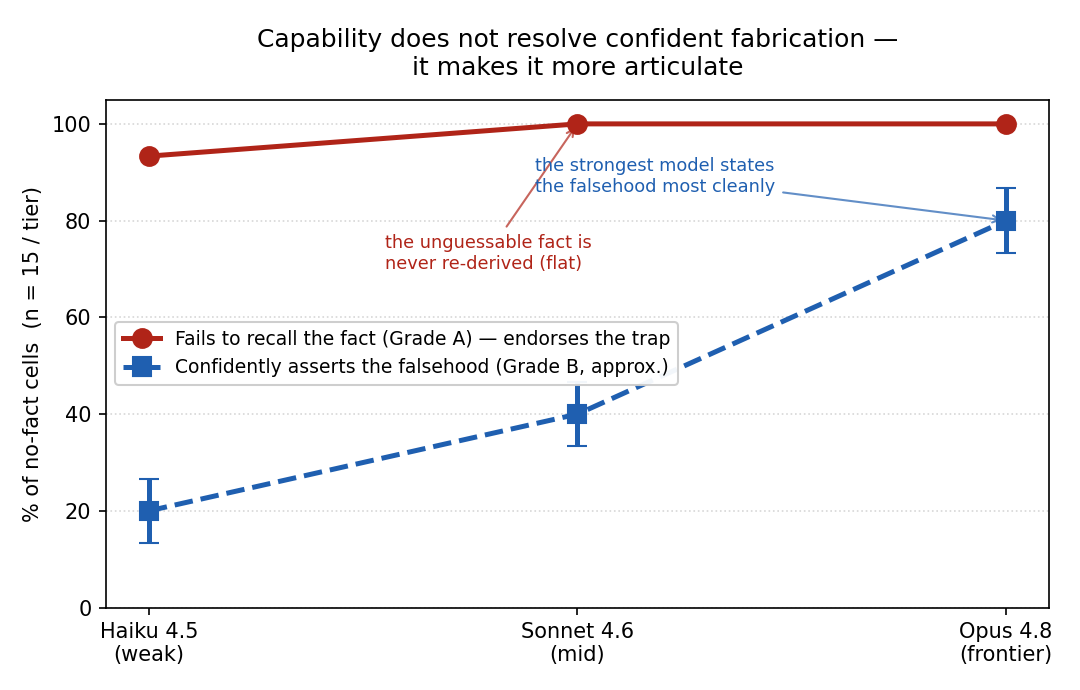
\includegraphics[width=\textwidth]{../../figures/calibration-gradient.png}
   \caption{Cross-scale calibration ($n = 15$ / tier), two independent runs. Failing to
   recall the hidden fact is flat at the ceiling---the fact is unguessable at every
   capability (robust). The ``confidently asserts the falsehood'' rate is \textbf{scoring-fragile}:
   run 1 (lenient) rises with capability, but run 2 (strict rerun) collapses at the top tier
   (12/15 $\rightarrow$ 0/15), because the strongest model pairs the false assertion with a ``verify it
   loaded'' step and often rejects the shortcut. There is no reliable capability gradient; the
   surviving claim is non-elimination, not ``stronger $\Rightarrow$ more confident'' (SOUL-142).}
   \label{fig:calibration}
   \end{figure}

\item \textbf{Token-scale and position depth test} --- \emph{done} (F038 needle at 8\%/50\%/92\% depth in a
   $\sim$6.6k-token record). No positional decay: 30/30 recall at every position, both models;
   middle (the worst case per [5]) as clean as primacy/recency. `Lost in the middle' did not
   appear at this scale for a \emph{semantically-unique} needle. This bounds the depth claim to
   the tested scale and a distinctive needle; arbitrary scale and a \emph{camouflaged} needle
   (needle-similar distractors, where [5] bites hardest) remain the standing residual.
\end{enumerate}

\section{Discussion}

The findings collapse onto one distinction. A meta-doctrine layer can try to make a
model \emph{reason better generically}, or it can \emph{carry information the model cannot
regenerate}. The first is reproduced, at equal compute, by an equivalent quantity of any
content---it is legibility, disposition, or compute, and it fades as the base model
improves. The second is not: a fact about a specific API, a convention specific to a
project, an incident specific to a team---these have no generic substitute, and they
remain decisive at the frontier. And the frontier failure mode is not benign: a capable
model that lacks the fact does not abstain; it can generate a confident, plausible,
wrong justification (Section 4.5)---the precise hazard against which an external,
unguessable anchor is the only defense. We resist the stronger claim that capability
\emph{monotonically} worsens this; our evidence is that capability does not \emph{resolve} it, and
that whether the strong or the weak model fails is gated by the form of the surviving
rule.

This reframes what such systems are \emph{for}. Their durable value is not a reasoning
prosthesis but a \textbf{memory of the unguessable}, plus the \emph{activation} scaffolding that
makes recording and checking reliably happen. The reasoning-ceremony---roles, councils,
forced perspectives, structured formats---reads like substance and measures like form.
That it reads like substance is not incidental: the same verbosity that makes it
\emph{feel} like better thinking is what a length-matched control reproduces.

The compression result sharpens the design rule. Because the dangerous failure is the
frontier model fabricating around a missing fact, an always-on rule-set must preserve
not just a rule's proposition but the \emph{force} of the counter-prior fact behind it; a
terse rule with the incident stripped invites the very fabrication it was meant to
prevent, and a loophole in the rule is the opening the strong model takes.

\section{Conclusion}

Most of what makes a meta-doctrine system \emph{feel} effective is the system making the work
legible and the model more verbose---reproduced, at equal compute, by semantically-empty
filler, and fading at the frontier. The part that genuinely changes what the model
decides is narrow and capability-robust: carrying project-specific, counter-default
knowledge the model cannot regenerate and a generic equivalent gets wrong, together with
the scaffolding that makes recording and checking reliably happen. \emph{Derivable dissolves;
unguessable persists.} A lean system that keeps the record, a small counter-default
rule-set, a tested skills catalog, and a firing completion gate---and cuts the
reasoning-ceremony to a line---captures the measured value at a fraction of the surface.

\section*{References}

\begingroup
\setlength{\parindent}{0pt}
\setlength{\parskip}{0.6em}

[1] M. Zheng, J. Pei, L. Logeswaran, M. Lee, D. Jurgens. \emph{When ``A Helpful Assistant'' Is
Not Really Helpful: Personas in System Prompts Do Not Improve Performances of Large
Language Models.} arXiv:2311.10054, 2023.

[2] D. Tran, D. Kiela. \emph{Single-Agent LLMs Outperform Multi-Agent Systems on Multi-Hop
Reasoning Under Equal Thinking Token Budgets.} arXiv:2604.02460, 2026.

[3] M. Gao, Y. Li, B. Liu, Y. Yu, P. Wang, C.-Y. Lin, F. Lai. \emph{Single-agent or
Multi-agent Systems? Why Not Both?} arXiv:2505.18286, 2025.

[4] T. Gan, Q. Sun. \emph{RAG-MCP: Mitigating Prompt Bloat in LLM Tool Selection via
Retrieval-Augmented Generation.} arXiv:2505.03275, 2025.

[5] N. F. Liu, K. Lin, J. Hewitt, A. Paranjape, M. Bevilacqua, F. Petroni, P. Liang.
\emph{Lost in the Middle: How Language Models Use Long Contexts.} arXiv:2307.03172, 2023.

[6] Y. Bai, S. Kadavath, S. Kundu, et al. \emph{Constitutional AI: Harmlessness from AI
Feedback.} arXiv:2212.08073, 2022.

[7] J. Kim, N. Yang, K. Jung. \emph{Persona is a Double-edged Sword: Mitigating the Negative
Impact of Role-playing Prompts in Zero-shot Reasoning Tasks.} arXiv:2408.08631, 2024.

[8] A. Kong, et al. \emph{Better Zero-Shot Reasoning with Role-Play Prompting.} NAACL 2024,
arXiv:2308.07702, 2024.

[9] Y. Du, S. Li, A. Torralba, J. B. Tenenbaum, I. Mordatch. \emph{Improving Factuality and
Reasoning in Language Models through Multiagent Debate.} arXiv:2305.14325, 2023.

[10] P. Lewis, E. Perez, A. Piktus, et al. \emph{Retrieval-Augmented Generation for
Knowledge-Intensive NLP Tasks.} NeurIPS 2020, arXiv:2005.11401, 2020.

[11] O. Ovadia, M. Brief, M. Mishaeli, O. Elisha. \emph{Fine-Tuning or Retrieval? Comparing
Knowledge Injection in LLMs.} EMNLP 2024, arXiv:2312.05934, 2023.

[12] OpenAI. \emph{GPT-4 Technical Report.} arXiv:2303.08774, 2023.

[13] S. Kadavath, T. Conerly, A. Askell, et al. \emph{Language Models (Mostly) Know What They
Know.} arXiv:2207.05221, 2022.

[14] J. Pfau, W. Merrill, S. R. Bowman. \emph{Let's Think Dot by Dot: Hidden Computation in
Transformer Language Models.} arXiv:2404.15758, 2024.

[15] F. Shi, X. Chen, K. Misra, et al. \emph{Large Language Models Can Be Easily Distracted by
Irrelevant Context.} ICML 2023, arXiv:2302.00093, 2023.

[16] J. Huang, X. Chen, S. Mishra, et al. \emph{Large Language Models Cannot Self-Correct
Reasoning Yet.} ICLR 2024, arXiv:2310.01798, 2023.

[17] C. Packer, S. Wooders, K. Lin, et al. \emph{MemGPT: Towards LLMs as Operating Systems.}
arXiv:2310.08560, 2023.

[18] J. S. Park, J. C. O'Brien, C. J. Cai, et al. \emph{Generative Agents: Interactive
Simulacra of Human Behavior.} UIST 2023, arXiv:2304.03442, 2023.

\endgroup

\bigskip

\emph{Citation provenance: [1]--[6] were resolved directly against arXiv during drafting;
[7]--[18] were fetched and adversarially cross-checked by a multi-agent literature sweep
(22 of 25 sampled claims confirmed, 3 refuted), then---in a final per-identifier sweep
(2026-06-05)---every one of [7]--[18] was re-fetched directly against arXiv and confirmed
correct on identifier, title, and authors (zero bad identifiers). That sweep did surface
two \textbf{venue} annotations that neither the arXiv page nor a targeted search could anchor---``[7]
EMNLP 2024 Findings'' and ``[14] COLM 2024''---which have been softened to arXiv-only
rather than asserted; venues that were confirmed are retained ([8] NAACL 2024 main, [11]
EMNLP 2024 main, [16] ICLR 2024, [18] UIST '23). This is a third reflexive instance of the study's own
anchor-validity discipline (cf.\ the TRiSM downgrade and the over-correction in \S6): an
unanchored attribution corrected at writing time rather than carried. The ``interpretability''
framing previously cited to a review paper (TRiSM, 2506.04133) remains downgraded to
background---see \S6.}

\bigskip

\emph{Companion blog (the narrative): \href{blog.md}{\texttt{blog.md}}. Consolidated result tables:
\href{data/results-tables.md}{\texttt{data/results-tables.md}}. The format-agnostic corpus this
paper renders---every probe's full design and data---is \href{00-method.md}{\texttt{00}}--\href{08-longitudinal-preference.md}{\texttt{08}}.}

\end{document}
